
\section{\texorpdfstring{Dusk Anonymous Network
Layer}{Dusk Anonymous Network Layer}}


In the vast majority of blockchain implementations, network
communication protocols limit themselves to just embracing the privacy
standards we have in place today for our daily internet needs: TCP/IP,
UDP, SSL for encrypting communication channels to name a few.

While this can be considered acceptable for centralized environments or
platforms where user privacy is not the main proposition, the anonymity
and privacy requirements established with the \textrm{Dusk} network impose the
adoption of technology offering a much higher level of privacy
protection.

To achieve this goal, \textrm{Dusk} is enabling full anonymity over its
decentralized network by integrating an advanced, custom bi-directional
routing, fully compatible with \href{https://geti2p.net/en/}{I2P}'s
\href{https://en.wikipedia.org/wiki/Garlic_routing}{Garlic-Routing}
technology for all its networking communications, but extending the
underlying protocol not only for the deployment of additional
functionality (such as fully anonymous file transfer) but also for
allowing the default anonymous gossip protocol which powers the entire
\textrm{Dusk} network.

The proposed architecture has been designed to make it computationally
infeasible for an eavesdropper to tell apart \textrm{Dusk} related traffic
from other network activities. Additionally, it should be very hard for
any network node to associate a \(Tx_{id}\) with the IP address of the
original initiator.

Compared to similar solutions, the \textrm{Dusk} approach offers the following
benefits:

\begin{enumerate}
\def\labelenumi{\arabic{enumi}.}
\item
  Makes use of \emph{packet routing}, instead of \emph{circuit routing}.
  This means transparent load balancing of all networking message across
  peers, instead of a single tunnel.
\item
  Multiple packets are joined together in inconspicuous messages, making
  it exponentially difficult for an attacker to expose network
  communications.
\item
  True decentralization: it uses a distributed directory to have an
  overview of the network, as opposed to relying on a centralized
  bulletin board.
\item
  Uni-directional tunnels guarantee that incoming and outgoing traffic
  is kept decoupled; a measure engineered to enhance transmission
  unlinkability through data stream separation. (Figure \ref{tunn})
\end{enumerate}

When negotiating access to the network, the accessor node (Alice)
selects \emph{Entry tunnel} to route (\emph{encrypted}) messages
through.

Each node in the network acts as a \emph{de facto} router, by relaying
the message multiple times, until it gets delivered to an \emph{Exit
Tunnel}, for which the last node has been chosen by the message
recipient (\emph{Bob}).

\subsection{Bootstrap}

Prior to forming the \emph{Entry Tunnel}, the accessor connects to a
blockchain's \emph{seed server} or \emph{vouching seeder} (inert network
nodes specifically designed to facilitate the bootstrap of peers by
relaying configuration parameters, the blockchain's current snapshot) in
order to obtain a list of active nodes. The \emph{vouching seeder}
replies with a message containing three parts:

\begin{enumerate}
\def\labelenumi{\arabic{enumi}.}
\item
  the collection of candidate entry node IPs
\item
  the collection of candidate entry node public keys and the public key
  of the accessor node
\item
  the seeder's signature of 2 and its public key
\end{enumerate}

The part 2. and 3. of the message are called the \emph{vouch}\\

\begin{figure}
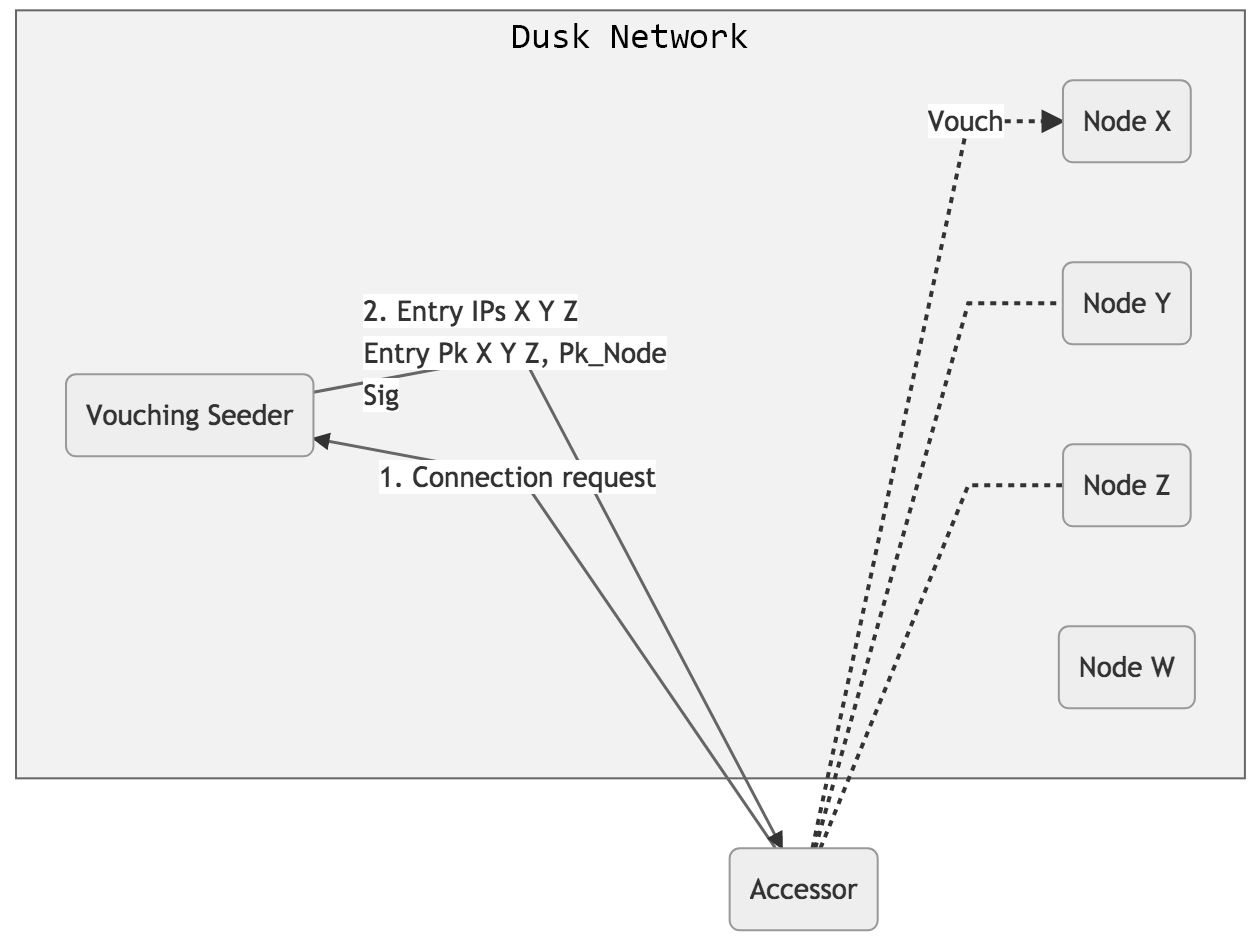
\includegraphics[scale=0.18]{bootstrap}
\caption{\textrm{Dusk} Network Bootstrap}
\label{boot}
\end{figure}

\begin{figure*}
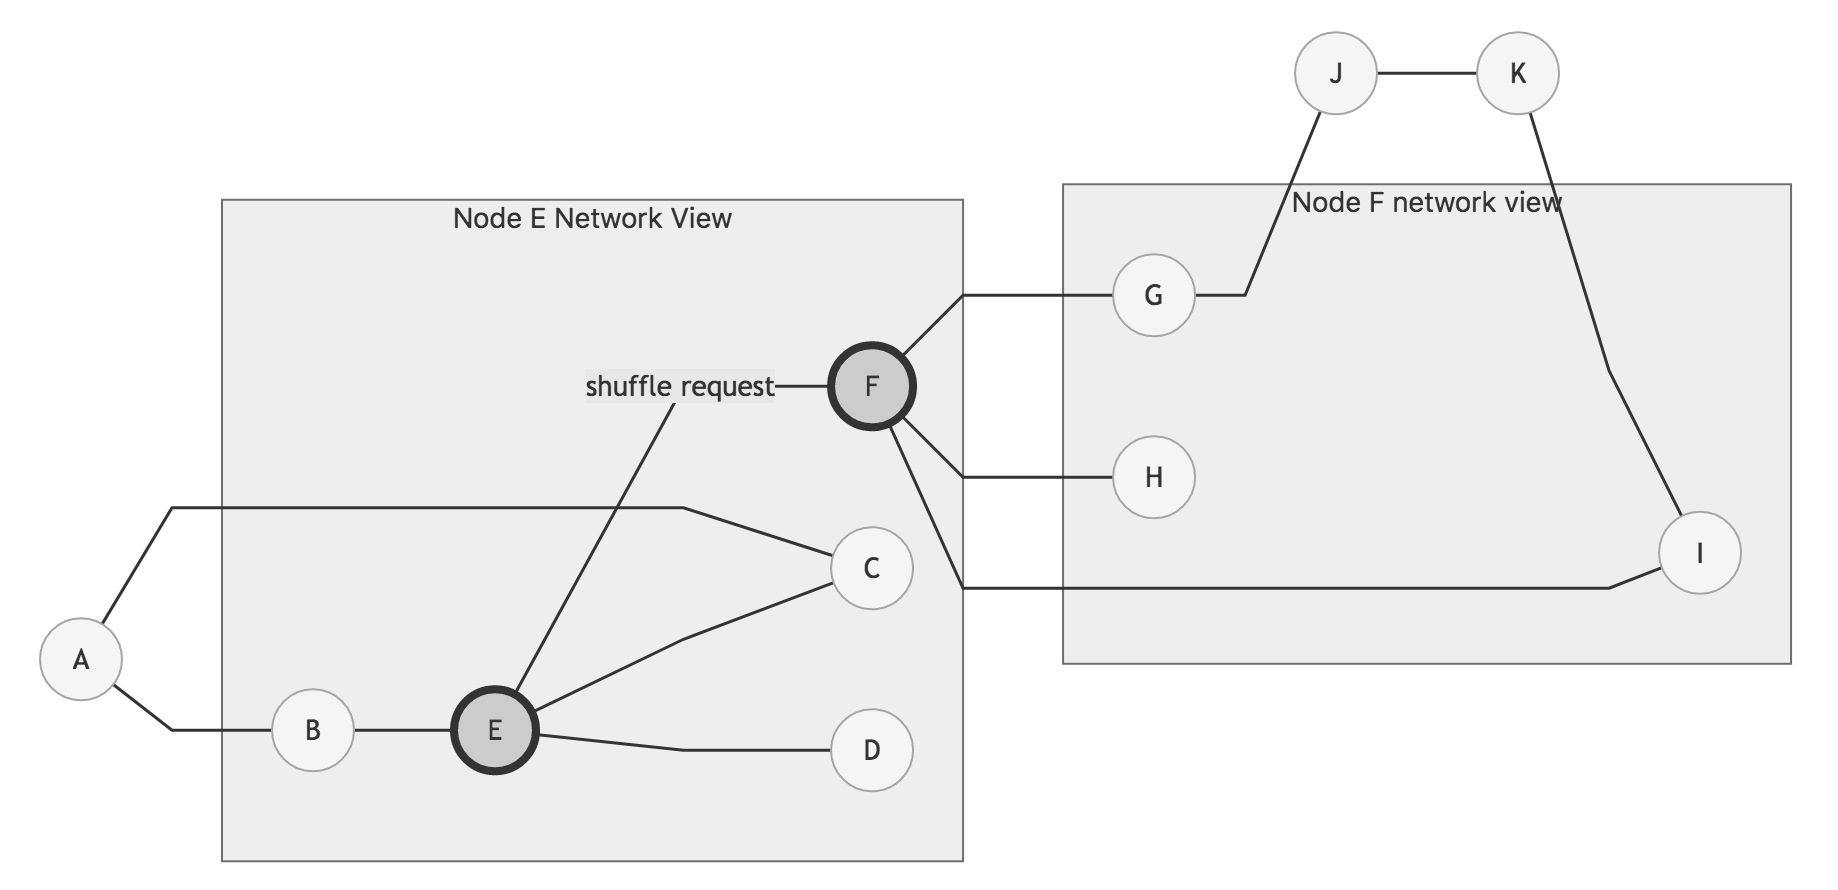
\includegraphics[scale=0.25]{gossip1}
\caption{Example gossip setup}
\label{goss1}
\end{figure*}


The accessor node thus selects an arbitrary end point \(X\) chosen among
those offered by the \emph{vouching seeder}. Thus, the accessor requests
\emph{Entry Tunnel} forming with \(X\) by sending the \emph{vouch} so
that \(X\) can verify the \emph{vouching seeder}'s signature and the
public key of the accessor, thus preventing potential IP routing leaks.
If the verification fails, the node refuses access, marks the node as
malicious and puts its IP into a distributed blacklist.

The accessor will then receive a set of active endpoints where
connection can be initiated, and will be assigned a hash which will act
as a mask for his real IP address. Similarly, the other nodes in the
network will be reachable solely through their own hash-mask. The
vouching seeders are trusted servers, reachable via a secured
\emph{https url} encoded into the \textrm{Dusk} main core.

\subsection{Gossip Communication}



Once connected to the arbitrarily selected \emph{Entry Node},
\emph{Accessor} will become a full fledged member of the \textrm{Dusk}
Network, and will receive from the \emph{Vouching Seeder} and the
\emph{Entry Node} an initial snapshot of \emph{\textrm{Dusk} addresses} it can
gossip to. This internal, partial view of the network is constantly
maintained and refreshed by using a \emph{peer-sampling service}, which
is itself gossip-based. By using this service, the node will
periodically ask other nodes for an updated view of the network, and
will receive in return a set of addresses to update its internal view
with. For efficient message spreading, it is also imperative that the
internal view of each node is as random as possible, and for this
reason the \emph{peer-sampling service} is also designed to maintain
high entropy within the network by occasionally shuffling nodes between
requesting peers.

Let's assume the structure in Figure \ref{goss1}, with nodes \(E\) and \(F\)
being two nodes about to shuffle addresses between each other.

In the scenario above, Node \(E\)'s internal node tables is
\([C, D, B, F]\) - which is the list of node addresses he knows about.
Node \(F\)'s internal node table will be instead \([G, I, H, E]\). When
shuffling nodes, the top of the head of each table is exchanged between
peers, so Node \(E\) will send to Node \(F\) the addresses \([C,B]\) and
in return will receive \([G,I]\). The new internal tables will modify
the network structure as in Figure \ref{goss2}.

\begin{figure*}
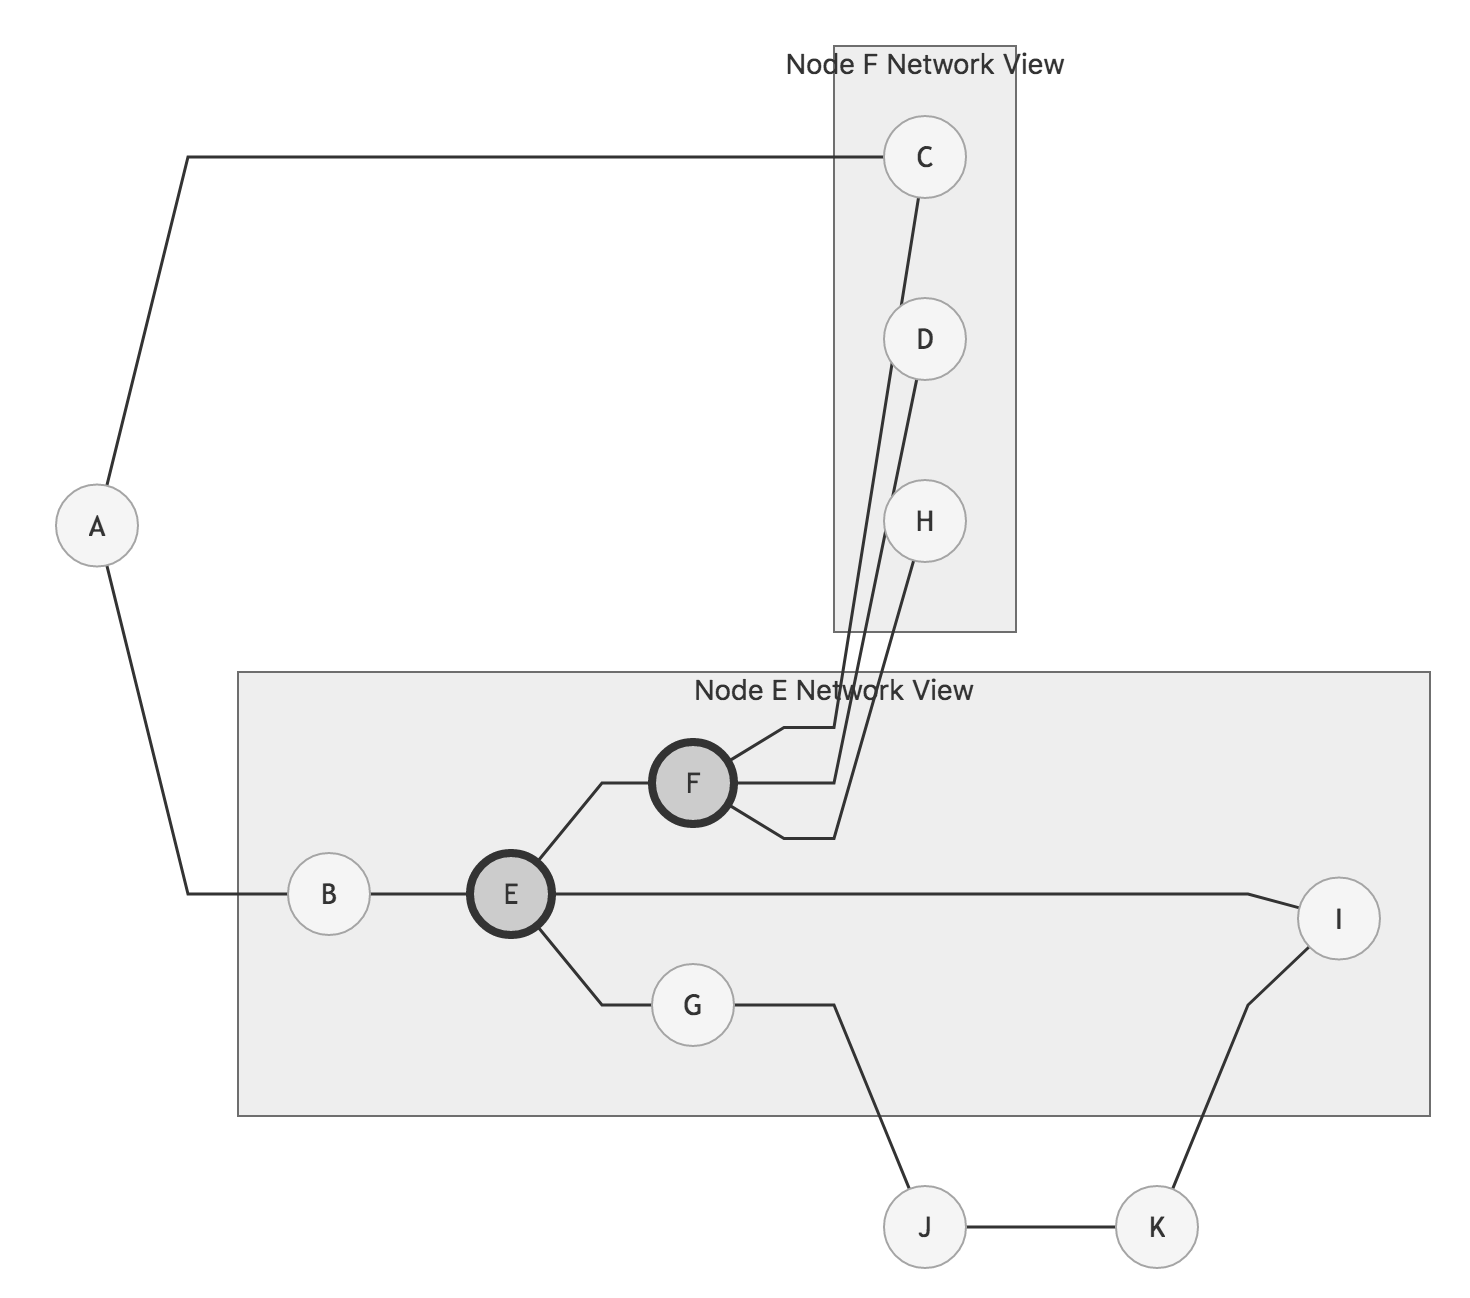
\includegraphics[scale=0.25]{gossip2}
\caption{Gossip setup post-shuffle}
\label{goss2}
\end{figure*}


This procedure ensures that configurations are never stagnant, and high
levels of randomness are always kept within the Network.


\subsection{Peer-Status Propagation}

Synchronising information about peer's \textrm{Dusk} addresses happens with a
gossip-based communication scheme, called Peer-Status Propagation, which
is slightly more involved than the one used for transaction propagation
(which resembles more a \emph{fire-and-forget} approach). Peer-Status
Propagation shows resemblance to a TCP three-way handshake and it is a
suitable scheme to synchronise information relating to peer-sampling
table, a list of recent Provisioners, new peers joining the network or
addresses consistently in timeout. Another possibility (not explored in
this paper) is to exchange information about responsiveness of different
peers in order to stipulate a constantly updated overview of convenient
low-latency routes.

\begin{figure}
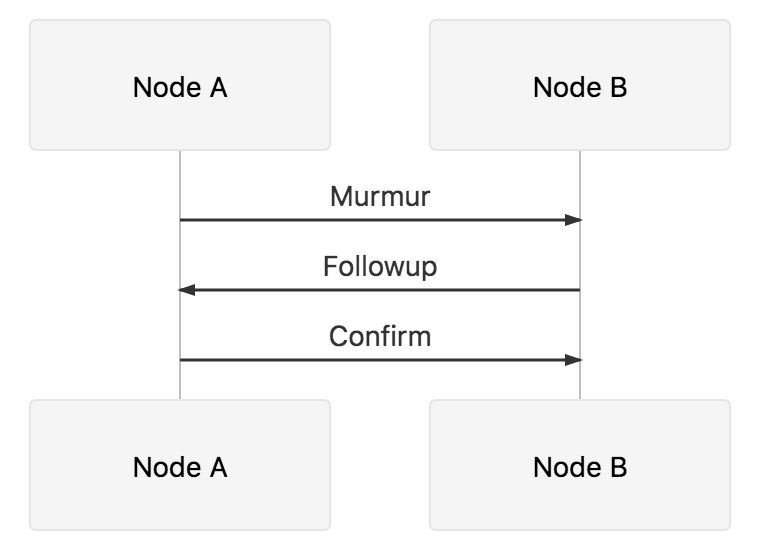
\includegraphics[scale=0.25]{peerprop}
\caption{Peer Status Propagation}
\label{peerprop}
\end{figure}

The information is exchanged as follows:

\textbf{Murmur} : The node initiating the communication sends out a
message to a receiving peer which contains his current view of the
network, plus information of the node itself (uptime, version), and
meta-data describing part of its internal status which he wishes to
transmit.

\textbf{Followup} : the receiving peer computes a difference between his
own meta-data and the one that was sent to it by the initiator. It then
follows up on the communication with a reply containing the gossip the
initiator ignores and a list of peer addresses the initiator does not
know about.

\textbf{Confirm}: After receiving the \emph{Followup} message, the
Initiator updates his meta-data with the message it just received by the
peer, saves the information, and sends out a \emph{Confirm} message with
the missing information the peer did not know about, if necessary. This
marks the end of the Status Propagation Round.

The increase of network traffic due to the Peer-Status Propagation is
constant and not expected to perceivably impact the efficiency of the
network. Relaying the \textbf{murmuring} is in fact limited to a
restricted number of peers (i.e. three/four nodes) and \emph{Stata}
synchronization happens through the constant 2-phases Followup and
Confirm messages without causing any network spike.
\begin{figure*}
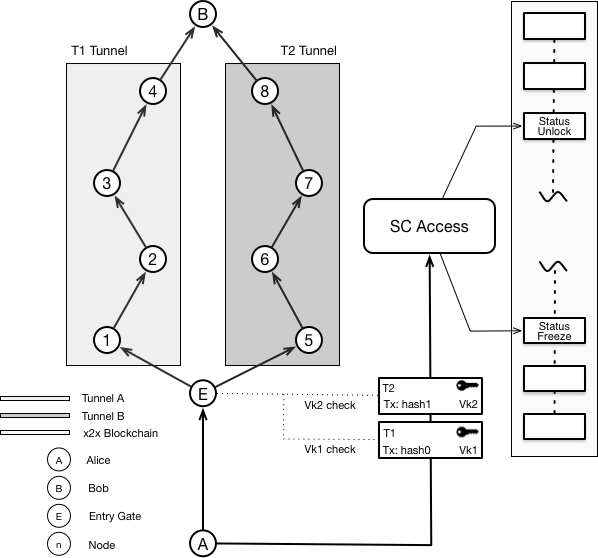
\includegraphics[scale=0.5]{tunnelswitch}
\caption{Tunnel Switching}
\label{tunnelswitch}
\end{figure*}
\subsection{Transaction Propagation}

The \textrm{Dusk} blockchain makes use of advanced gossip network technology
in order to propagate transactions and sortition results for Block
Generator/Validators. Gossip protocols follow the \emph{endemic} message
dissemination system and represent a natural fit for a P2P network needing to frequently synchronize small status variations among its peers
through the following advantages:

\begin{itemize}
\item
  \textbf{Scalability}: The general complexity of
  \href{https://pdfs.semanticscholar.org/3df0/523ff58d8dec53e89a521831265af32f52d6.pdf}{network
  gossip protocols}, is
  \href{https://arxiv.org/pdf/1512.03022.pdf}{\(O(logN)\)} which
  represents the number of rounds to reach all nodes in the network,
  where \(N\) is the total number of nodes. Nodes only send a limited
  number of messages and do not wait for acknowledgements. Such a system
  can easily scale although it cannot achieve unbound scalability given
  the requirement of achieving global dissemination. In the case of
  the \textrm{Dusk} Blockchain, there is an inherent partition of nodes given by
  the fact that messages around block proposals, validations and voting
  is performed solely by Provisioners which relay these messages solely
  to other Provisioners.
\item
  \textbf{Error Tolerant}: \textrm{Dusk} can operate extremely well with
  unreliable connections and unorthodox configurations. The same packets
  are sent multiple times to different peers - this way, should an
  infrastructure problem arise between two points impeding their
  communication, they will both receive the same message from other
  nodes in the network.
\item
  \textbf{Decentralization Ready}: There is no central role for any of
  the nodes. Each node works as an independent agent, with
  pre-established rules about data transmission.
\end{itemize}



A desirable property the \textrm{Dusk} gossip protocol is obtaining relatively
low complexity while guaranteeing safety. For this reason, nodes
in the network do not relay more than one message/transaction coming
from the same node per \(\langle step, round \rangle\) of
\emph{SBA}\(\large\star\).

When a node wants to transmit information (transactions, sortition
results, etc.) it selects \(n\) random nodes from the set of nodes it
knows about (through the \emph{peer sampling service}) and transmits
such information to them, who, in turn, relay it further. Information
gets periodically sent to \(N\) targets, where \(N\) is known as the
\emph{Fanout}.

With \(Fanout=1\), we will need \(O(log N)\) \emph{Cycles} (which is the
number of rouds to spread a rumor) for the information to reach all
nodes.

In order to safeguard the anonymity of the peers, most of the messages
are relayed through anonymous datagrams following the specification of
I2P's \href{https://geti2p.net/spec/datagrams}{Non-Repliable Datagram},
which are packets devoid of sender \texttt{IP} information using the
\texttt{UDP} protocol. In the first instance of the \textrm{Dusk} network, we
will make use of \href{https://geti2p.net/el/docs/api/samv3}{SAM v3}
protocol before considering rolling out a custom-made solution (which
might be necessary in case \textrm{Dusk} will need to relay packets bigger
than 32Kb).




\section{Secure Tunnel Switching (STS)}

Powered by the \textrm{Dusk} Blockchain, the \textrm{Dusk} Network layer aims to
provide a next-generation, cryptographically secure way to perform
secure audio, video and data streaming between two distinct nodes on the
network. Current technologies limit themselves estaablishing a secure
connection between peers - but the \textrm{Dusk} approach we are about to
describe goes far beyond that, by making sure that even if a node of the
network becomes compromised, the overall security of the platform as a
whole remains untouched.

\subsection{Setup}

We assume that node \emph{A} (Alice) wants to establish a secure data
stream connection with node \emph{B} (Bob), for which it knows the
relevant \textrm{Dusk} address. Before initiating any connection attempt, node
\emph{A} will commit a payment towards a \emph{Smart Contract Access
Point (SCAP)} at instant \(T_1\), using an off-chain transaction, for a
dynamic value that will be auto-regulated by the \textrm{Dusk} core. This is
done to keep the transmission cost stable, and also independent from
token fluctuations.

By receiving the transaction request, the \emph{SCAP} will freeze the
status on a block on the \textrm{Dusk} chain for node \emph{A} - to be updated
later when the off chain transactions will come to an end.

Upon finalizing the transaction, node \emph{A} will contact her entry
point \emph{E}, and provide it with the \emph{view key} as proof of
payment. In turn, \emph{E} will check the validity of the key, and if
correct will allow the opening of a \emph{garlic routing tunnel} for a
duration of time \(\Delta_T\) towards node \emph{B}, so that node
\emph{A} can initiate the transmission.

At instant \(\Delta_T + \frac{\Delta_T}{2}\), node \emph{A} will start a
new transaction with \emph{SCAS} to renew the duration of such tunnel
for an additional interval \(\Delta_T\), and if successful will open a
new tunnel with \emph{B}, and will start sending a concurrent, identical
data stream on the new one. Node \emph{B} will consequentially drop the
previous tunnel using a procedure that we will describe below. This
process will continue until the data transmission will
come to an end, by either \emph{A} choosing to not renovate a tunnel or
failing to complete a new transaction with the \emph{SCAP}.

If node \emph{A} does not provide her Entry point \emph{E} with a valid
view key for the next transaction, the tunnel will be dropped entirely
from the Entry point itself.

\subsection{Tunnel Switching}

Once it has received the data stream from sender node \emph{A}, receiver node
\emph{B} will parse the raw data (which can be a VoIP call, for example)
and will keep waiting for new tunnel connections. Upon receiving a
second connection, \emph{B} will match the two data streams by doing a
trivial bit matching operation, which will almost certainly show a small
time lag due to the fact that the two tunnels use a different set of
relaying nodes. (Figure \ref{datamatch})

\begin{figure}
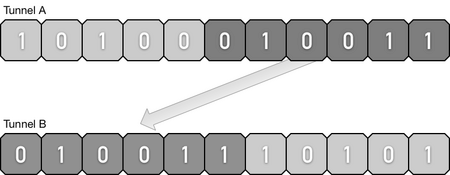
\includegraphics[scale=0.5]{dataswitch}
\caption{Data Match + Switch}
\label{datamatch}
\end{figure}

After successfully matching the streams, node \emph{B} can safely
discard the old one, and continue parsing the stream on the most recent
one. The procedure will repeat for as long as sender node \emph{A}
renews the transaction costs with the \emph{SCAS} to keep streaming data.

This dramatically improves security and anonimity over
a conventional \emph{Garlic Tunnel} connection. By switching the data
tunnel at regular intervals, a malicious attacker would be unable to
predict compromised nodes, perform DDoS attacks, and in general exploit
vulnerabilities on the network.

\section{On- Offline File Transfer}

The capability to anonymously and securely send files over the network and allow both offline and online retrieval is a unique feature of the \textrm{Dusk} Network. To implement such a use-case, \textrm{Dusk} combines the capabilities of the anonymous peer discovery and gossip mechanism previously described with those of a third party decentralized and anonymous storage service (e.g. the \href{https://orc.network/}{Orc Object Storage}). The workflow to securely send a file over the network is as follows:

\begin{itemize}
\item Alice encrypts file.doc using either Bob's \(P_k\) (in case the file is of modest size) or using a symmetric scheme such as AES-256 with key \(A_k\) to allow for better performances.
\item Alice will upload the file to the decentralized storage and will get the \texttt{id} of the file once the upload is complete. 
\end{itemize}

Alice will create an Anonymous Non-Repliable Datagram with the following structure:

\begin{center}\rule{0.5\linewidth}{\linethickness}\end{center}

\texttt{1:\ T7CvGQr0/nq8xiLfekdTUGz6rQggGnYYOxuXrMf4vPw=}\\
\texttt{2:\ GT7RzkvXJIPjT0xpJXVIhu6QjIzElxKDuvcJKyguwK3HT6GZaRA\\9/O4+XCKF67wNeyTfn8RGPM53lp0z+MLW2w==}\\
\texttt{3:\
PTlsG6c9kuDyU5vF91SMFAWe55GUi2Pxby+wgb9QYRhvCq5GIUp\\
dhA==} 

\begin{center}\rule{0.5\linewidth}{\linethickness}\end{center} \begin{figure} 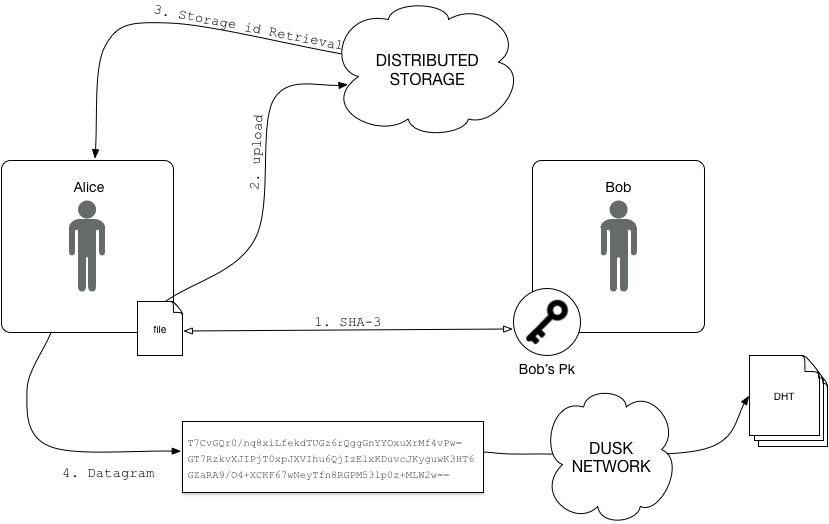
\includegraphics[scale=0.20]{orc} \caption{Secure File Transfer} \label{orc} \end{figure} The first line of the datagram is the encrypted \texttt{id} of the file on the decentralized storage (using Bob's \(p_k\)) and will be used to retrieve such file. Second line is Bob's \textrm{Dusk} Address, also encrypted with using Bob's \(p_k\). Third line is optional and is Alice's symmetric key encrypted with Bob's \(p_k\). This is needed in case symmetric encryption was chosen to encrypt the document. Fourth line is also optional and used in case Alice would like Bob to know she was the sender of the file, in which case she will add her own \textrm{Dusk} address, also encrypted using Bob's \(p_k\).

We will now have two separate cases, since Bob can be online when the file is sent, or offline.

\begin{itemize}
\item
  Bob is \textbf{online} --- Bob receives Alice's datagram, checks if he is the owner of the file by trying to decrypt the second line with his private key \(s_k\). If successful will also decrypt the first line and download the file at the location specified by the ID.
\item
  Bob is \textbf{offline} --- The entry will be inserted in a distributed hash table (DHT) and kept there for 30 days, which Bob can interrogate as soon as he is online in order to check for files that were addressed to him while he was away. The DHT will be supported by extending the \emph{Provisioner} protocol with a simplified version of the RPC primitives of \href{http://xlattice.sourceforge.net/components/protocol/kademlia/specs.html\#protocol}{Kademlia Specifications} implemented over Non-Repliable Datagrams.
\end{itemize}